\documentclass[a11paper]{article}

\usepackage{karnaugh-map}
\usepackage{subcaption}
\usepackage{longtable}
\usepackage{tabularx}
\usepackage{titlepage}
\usepackage{document}
\usepackage{booktabs}
\usepackage{multicol}
\usepackage{float}
\usepackage{varwidth}
\usepackage{graphicx}
\usepackage{appendix}
\usepackage{pifont}
\usepackage[usenames,dvipsnames]{xcolor}

\title{Devis de conception}

\class{Architecture et organisation des ordinateurs}
\classnb{GIF310}

\teacher{Marc-André Tétrault}

\author{
  \addtolength{\tabcolsep}{-0.4em}
  \begin{tabular}{rcl} % Ajouter des auteurs au besoin
      Benjamin Chausse & -- & CHAB1704 \\
      Shawn Couture    & -- & COUS1912 \\
  \end{tabular}
}

\newcommand{\todo}[1]{\begin{color}{Red}\textbf{TODO:} #1\end{color}}
\newcommand{\note}[1]{\begin{color}{Orange}\textbf{NOTE:} #1\end{color}}
\newcommand{\fixme}[1]{\begin{color}{Fuchsia}\textbf{FIXME:} #1\end{color}}
\newcommand{\question}[1]{\begin{color}{ForestGreen}\textbf{QUESTION:} #1\end{color}}

% Checkboxes
\setlength{\fboxsep}{1pt}
\newcommand{\cbox}{\fbox{\phantom{\ding{51}}}}
\newcommand{\cboxtick}{\fbox{\ding{51}}}%

% self-incrementing Test-ID
\newcounter{tid}
\newcommand{\tid}{\stepcounter{tid}\thetid}

\renewcommand{\frenchtablename}{Tableau}

\newcommand{\vtt}[1]{%
  \text{\normalfont\ttfamily\detokenize{#1}}%
}


\begin{document}
\maketitle
\newpage
\tableofcontents
\newpage

\section{Spécifications SIMD sommaires}

De la même façon que l'architecture MIPS contient 32 registres de 32 Bits, les
nouvelles instructions SIMD introduisent 32 nouveaux registres de 128 Bits
($4\times32$ Bits). De cette façon, chaque opération SIMD peut accéder à des
registres de la même façon que le font les autres opération sans pour autant
entrer en conflit avec celles-ci et les corrompres. Aussi, un nouveaux type
d'instruction n'a pas besoin d'être créé (autre que \verb|R|,\verb|I|,\verb|J|)
puisque les nouvelles instructions SIMD peuvent suivre la même structure.

Puisque la nouvelle architecture est spécifiquement nécessaire pour optimiser
le temps d'éxécution de l'algorithme viterbi, des instructions ont été faites
spécifiquement pour cette situation. Par exemple, viterbi n'opère pas sur des
chiffres négatifs. Ainsi, les opérations \verb|addv| et \verb|minv| plus bas
opèrent sur des entiers non-signés.

\subsection{lwv: Load word vector}

L'opération prends comme premère opérand un registre de type vectoriel
(\verb|$zn| désignerait le nième registre) ainsi que l'adresse mémoire du
premier mot. Le processeur prends ensuite 4 mots contigus en mémoire en prenant
l'adresse fournie comme première et les stockent dans un seul registre de
128Bits.

\subsection{swv: Store word vector}

Cette opération effectue le contraire de \verb|lwv|, prenant le contenu d'un
registre vectoriel fourni comme premier opérand, le séparant en 4 mots
distincts puis stockant chacun de ces mots dans la mémoire. Ce stocakge se fait
en commençant par l'addresse mémoire fournie en deuxième opérand pour le
premier mot puis les autres un à la suite des autres.

\subsection{addv: Add vectors}

L'opération \verb|addv $z0, $z1, $z2| faits la somme du vecteur \verb|$z1| et
\verb|$z2| pour ensuite stocker le résultat dans le registre vectoriel
\verb|$z0|. En considérant que \verb|$zn[0]| correspond au premier mot stocké
dans le registre $n$, le calcul est effectué de la façon suivante:

\begin{align}
  \vtt{$z0[0]} &= \vtt{$z1[0]} + \vtt{$z2[0]} \\
  \vtt{$z0[1]} &= \vtt{$z1[1]} + \vtt{$z2[1]} \\
  \vtt{$z0[2]} &= \vtt{$z1[2]} + \vtt{$z2[2]} \\
  \vtt{$z0[3]} &= \vtt{$z1[3]} + \vtt{$z2[3]}
\end{align}

\subsection{minv: Minimum within vector}

Cette instruction est particulière puisqu'elle fait interagir des registres
vectoriels avec des registres normaux de la façon qui suit. Le deuxième opérand
fourni correspond à un registre vectoriel. L'opération détermine lequel des 4
mots contenu à l'intérieur de ce vecteur a la plus petite valeur et stocke ce
résultat dans le registre normal fourni en premier opérand. Ainsi avec le
registre vectoriel \verb|$z0 = {4,1,2,3}|, l'opération \verb|minv $t0, $z0| va
stocker la valeur $1$ dans le registre temporaire \verb|$t0|.

\section{Plan de vérification}

Puisqe le but premier des procédures qui suivent est de s'assurer que des
actions prédéfinies donnent des résultat prévus (et non de jouer à où est
Charlie), chaque appel à la mémoire (\verb|lw|, \verb|sw|, \verb|lwv|,
\verb|swv|) vont agir sur des addresses prédéfinies dans le `.data` du
programme. Ces addresses peuvent être retrouvées dans le tableau \ref{tab:data}
de l'Annexe.

D'autre part, le tableau \ref{tab:vars} contient des valeurs de résultats
attendues.
L'ordre des tests est particulièrement important puisque plusieurs tests
dépendes du succès des tests précédents.

Aussi, afin de s'assurer que les changements apporté à l'architecture n'ont pas
affecté le bon fonctionnement de l'infrastructure déjà en place, les premiers
tests servent d'assurance à cet effet.

\begin{center}
  \begin{longtable}{lp{5cm}p{3.5cm}p{4.5cm}l}
		% Headers & Footers {{{
		\caption{Plan de vérification} \label{tab:verif}
		\\

		\toprule
		\multicolumn{3}{l}{Objectif Ciblé} &
		\multicolumn{2}{l}{Test des nouvelles opérations}
		\\

		\midrule
		\#                         &
		\bfseries Test             &
		\bfseries Action           &
		\bfseries Résultat Attendu &
		\cboxtick
		\\

		\midrule
		\endfirsthead

		\multicolumn{5}{c}%
		{{\itshape \tablename\ \thetable{} -- Continué de la page précédente\ldots}}
		\\

		\midrule
		\#               &
		Test             &
		Action           &
		Résultat Attendu &
		\cboxtick
		\\

		\midrule
		\endhead

		\midrule \multicolumn{5}{r}{{Continué à la prochaine page}}
		\\
		\midrule
		\endfoot

		\bottomrule
		\endlastfoot
		% }}}
		\tid & \verb|lw|:
		"Load Word" fonctionne toujours                  &
		\verb|lw base_val, $t4| &
		Le registre unitaire \verb|$t4| devrait contenir \verb|0xdead| &
		\cbox
		\\

		\tid & \verb|sw|:
		"Store Word" fonctionne toujours                  &
		\verb|sw $t4, $t4| &
		L'addresse \verb|out_norm| devrait contenir \verb|0xdead| &
		\cbox
		\\

		\tid & \verb|add|:
		L'arithmétique sur des registres standards fonctionne toujours &
    \verb|lw $t5 base_add|
		\verb|add $t6, $t4, $t5|
    \verb|sw $t6, sum_norm| &
		L'addresse \verb|sum_norm| devrait contenir \verb|0x19d9c| &
		\cbox
		\\

		\tid & \verb|lwv|:
		Il est possible de stocker de la mémoire vers des registres vectoriels &
		\verb|lwv $z0, ben_vec|                &
    Le registre vectoriel \verb|$z0| devrait contenir la même chose que
    \verb|ben_vec| (avec les valeurs dans le même ordre)
    et l'opération \verb|lwv| ne devrait prendre qu'un seul coup d'horloge &
		\cbox
		\\

		\tid & \verb|swv|:
		Il est possible de stocker d'un registre vectoriel vers la mémoire &
		\verb|swv $z0, out_vec|                &
    L'addresse \verb|out_vec| devrait contenir la même chose qu'à
    l'addresse \verb|ben_vec| et l'action de stockage ne devrait prendre qu'un
    coup d'horloge &
		\cbox
		\\

		\tid & \verb|addv|:
		Il est possible de stocker la somme de deux registres vectoriels dans un troisième
    registre &
		\verb|lwv $z1, lower_vec|
		\verb|add $z2, $z0, $z1|
		\verb|swv $z2, out_vec|
    &
    L'addresse \verb|out_vec| devrait contenir la même chose que \verb|Vsum|
    et l'opération \verb|addv| ne devrait prendre qu'un seul coup d'horloge &
		\cbox
		\\

		\tid & \verb|minv|:
		Il est possible de stocker la valeur minimale d'un registre vectoriel à l'index 0 dans
    un registre unitaire &
		\verb|minv $t0, $z0|
		\verb|lw  $t0, min_val|
    &
    L'addresse \verb|min_val| devrait contenir \verb|'B'|
    et \verb|minv| ne devrait prendre qu'un seul coup d'horloge &
		\cbox
		\\

		\tid & \verb|minv|:
		Il est possible de stocker la valeur minimale d'un registre vectoriel à l'index 1 dans
    un registre unitaire &
		\verb|lwv $z3, min_one|
		\verb|minv $t0,  $z3|
		\verb|sw  $t0, min_val|
    &
    L'addresse \verb|min_val| devrait contenir  contenir 1
    &
		\cbox
		\\

		\tid & \verb|minv|:
		Il est possible de stocker la valeur minimale d'un registre vectoriel à l'index 2 dans
    un registre unitaire &
		\verb|lwv $z3, min_two|
		\verb|minv $t0,  $z3|
		\verb|sw  $t0, min_val|
    &
    L'addresse \verb|min_val| devrait contenir  contenir 2
    &
		\cbox
		\\

		\tid & \verb|minv|:
		Il est possible de stocker la valeur minimale d'un registre vectoriel à l'index 3 dans
    un registre unitaire &
		\verb|lwv $z3, min_three|
		\verb|minv $t0,  $z3|
		\verb|sw  $t0, min_val|
    &
    L'addresse \verb|min_val| devrait contenir  contenir 3
    &
		\cbox
		\\

	\end{longtable}
\end{center}

\section{Figure d'organisation}

\begin{figure}[H]
  \centering
  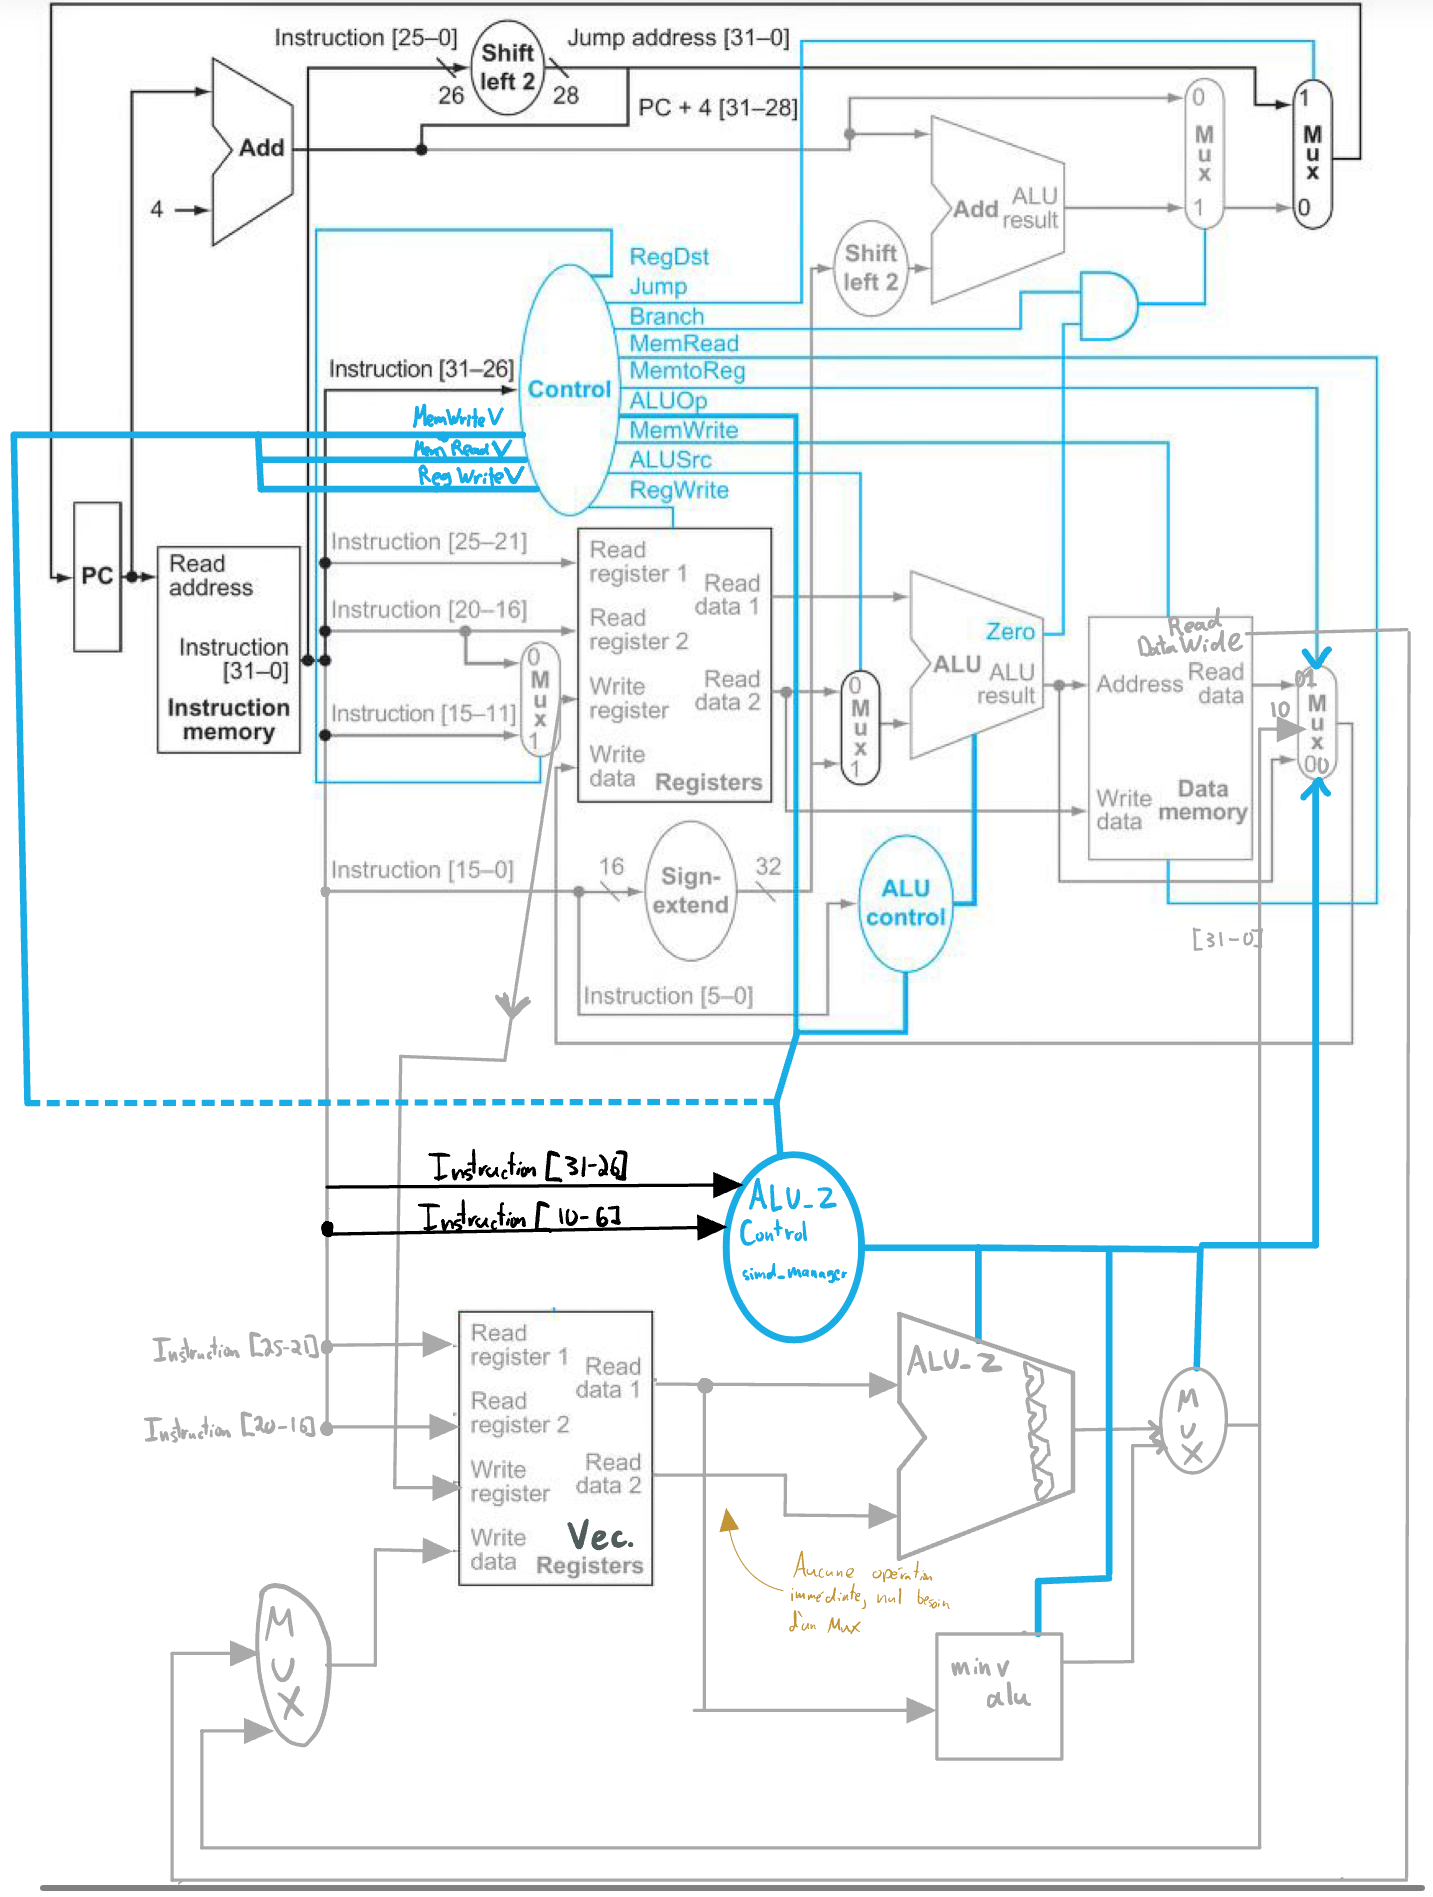
\includegraphics[width=.7\textwidth]{assets/bloc.jpeg}
  \caption{Schéma bloc du processeur à jour avec les instructions SIMD}
  \label{fig:bloc-diagram}
\end{figure}

\begin{appendices}
\section{Valeurs utiles}

\begin{table}[H]
	\centering
	\footnotesize
	\caption{Valeurs initiales de diverses addresses dans le programme du plan de vérification}
	\label{tab:data}
	\begin{tabular}{@{}cp{5.5cm}l@{}}
		\toprule
    \textbf{Nom} &
    \textbf{Valeur(s)} hex/déc./ASCII selon le besoin &
    \textbf{Description} \\
		\midrule

    \verb|base_val|  & \verb|0xdead|               & Mot pour tester le stockage unitaire dans un registre        \\
    \verb|base_add|  & \verb|0xbeef|               & Deuxième mot unitaire (pour tester une somme)                \\
		\verb|out_norm|  & \verb|0|                    & Emplacement pour tester un stockage unitaire                 \\
		\verb|sum_norm|  & \verb|0|                    & Emplacement pour stocker le résultat de la somme unitaire    \\
		\verb|ben_vec|   & \verb|{'B', 'E', 'N', 'C'}| & Vecteur pour tester le stockage dans un registre             \\
		\verb|lower_vec| & \verb|{32,32,32,32}|        & Vecteur de offset entre un Majuscule et Minuscule ASCII      \\
		\verb|out_vec|   & \verb|{0,0,0,0}|            & Endroit pour tester le stockage de vecteurs                  \\
    \verb|min_one|   & \verb|{4,1,2,3}|            & Vecteur ayant sa valeur minimale à l'index 1 \\
    \verb|min_two|   & \verb|{4,5,2,3}|            & Vecteur ayant sa valeur minimale à l'index 2 \\
    \verb|min_three| & \verb|{4,5,6,3}|            & Vecteur ayant sa valeur minimale à l'index 3 \\
		\verb|min_val|   & \verb|0|                    & Endroit pour stocker le résultat d'une opération \verb|minv| \\

		\bottomrule
	\end{tabular}
\end{table}

\begin{table}[H]
	\centering
	\footnotesize
	\caption{Valeurs initiales de diverses addresses dans le programme du plan de vérification}
	\label{tab:vars}
	\begin{tabular}{@{}cp{5.5cm}l@{}}
		\toprule
    \textbf{Nom} &
    \textbf{Valeur(s)} hex/déc./ASCII selon le besoin &
    \textbf{Description} \\
		\midrule

    $\vtt{Rsum}$ & \verb|0x19d9c|              & Somme attendue de \verb|0xdead + 0xbeef| \\
    $\vtt{Vsum}$ & \verb|{'b', 'e', 'n', 'c'}| & Somme attendue de \verb|{'B','E','N','C'} + {32,32,32,32}| \\

		\bottomrule
	\end{tabular}
\end{table}

\end{appendices}

\end{document}
